\chapter{Genome assembly of Candida nivariensis}
\label{chap:rnw}





This document was generated on Mon May  2 14:39:59 2022.

As shown in Figure \ref{fig:myfig} and in Table \ref{tab:rtab1} we can see that bla bla \citep{B}.


\begin{figure}[!ht]
\centering
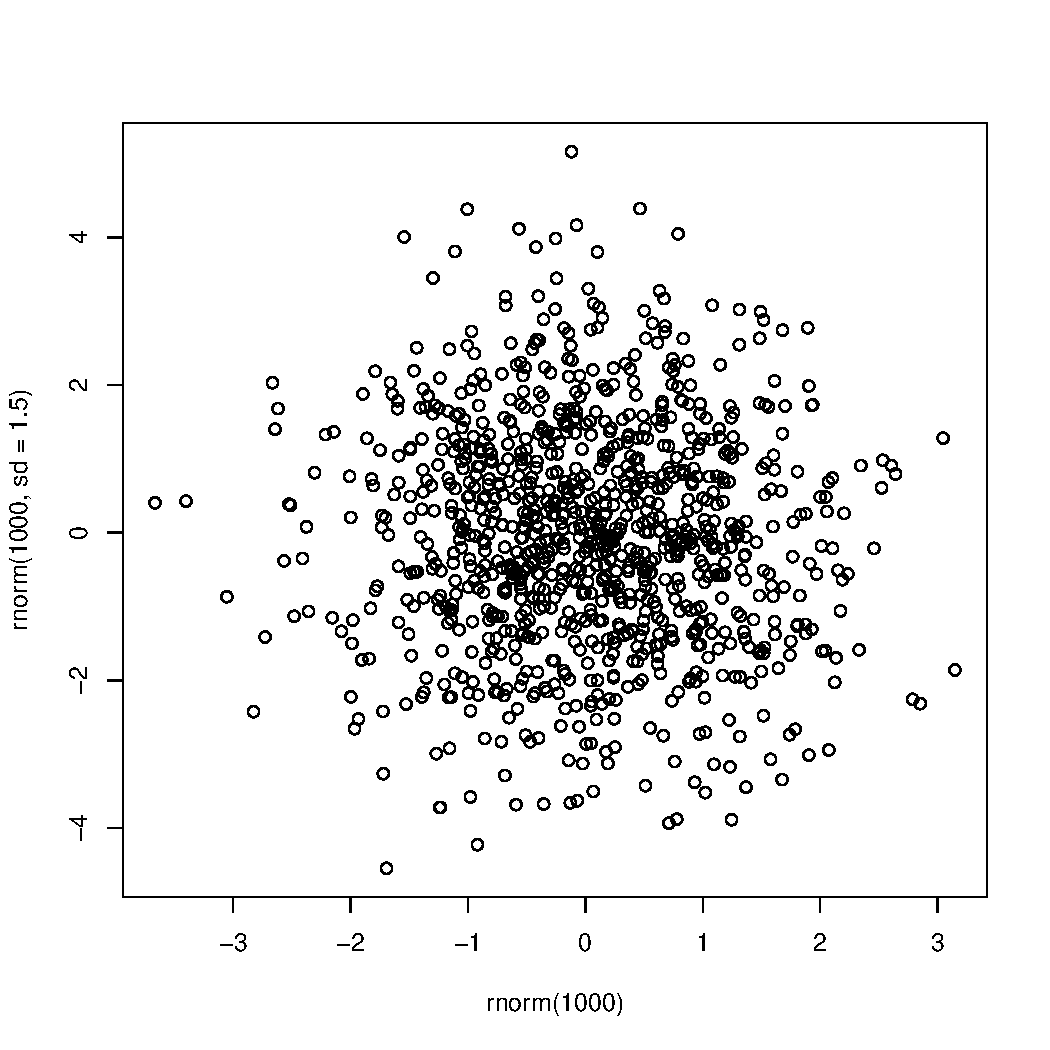
\includegraphics[width = 1\linewidth,keepaspectratio]{figure/myfig.pdf}
\caption[Some random figure]{{\bf Some random figure.} {\bf (a)} blah first point {\bf (b)} blah second point {\bf (c)} blaih thrid panel  }
\label{fig:myfig}
\end{figure}




% latex table generated in R 3.6.3 by xtable 1.8-4 package
% Mon May  2 14:39:59 2022
\begin{table}[ht]
\centering
\begin{tabular}{rr}
  \hline
A & B \\ 
  \hline
  1 & -1.01 \\ 
    2 & -1.46 \\ 
    3 & 0.13 \\ 
    4 & -0.17 \\ 
    5 & 0.40 \\ 
    6 & -0.00 \\ 
    7 & -1.34 \\ 
    8 & 0.31 \\ 
    9 & 0.29 \\ 
   10 & 0.49 \\ 
   \hline
\end{tabular}
\caption{\bf{ Table title } Table description} 
\label{tab:rtab1}
\end{table}

